\section{Educational Games for Private Consumers}
\label{sec:privateconsumers}
Many companies create educational games for children to learn math, languages and other basic school topics.
Most of these games are targeted towards younger children, who are about to start school or are in elementary school.
A company like Krea Games \cite{kreagames} creates multiple series for differently aged children.
These games are mostly available for PC, with a small subset also being available for Android and iOS devices.
In the following subsection we will examine some of the best selling educational games for private consumers, explain why we feel they are good games and how features of these games can be used in combination with our product.\todo{Make sure that we relate below discussion to final product.}

\subsection{Best Selling Educational Games}
One of the most popular educational games is The Oregon Trail, released first in 1982 with more than 65 million copies sold worldwide since.\cite{oregontrail}
The objective in the game is to help a family of American pioneers follow the Oregon Trail and help them survive their endeavor and settle down in Oregon.
The game The Oregon Trail intends to teach children about the life of the pioneers on the Oregon Trail in the middle of the 19th century.
The game manages to teach children the history of the Oregon Trail without sacrificing the gameplay experience, and thus the game is considered a good game even without the educational aspect.\newline

Other popular educational games are:
\begin{itemize}
	\item Where in the World Is Carmen Sandiego? from 1985 with many sequels released as late as 1998.\cite{carmensandiego}
	\item A facebook version of the first game was released in 2011.
	\item Lemonade Stand created by Bob Jamison in 1973.\cite{lemonadestand}
\end{itemize}

The game Where in the World Is Carmen Sandiego? teaches geography by making the player follow clues to where in the world a thief they need to catch has gone.
Later games in the series teach different subjects such as history or math.
Lemonade Stand is a game where the user play a child that has a lemonade stand.
The player has to make choices regarding the cost of the lemonade, money spent on advertising and how many glasses of lemonade to make.
The game teaches basic economics without feeling like schoolwork. Instead the player needs income to continue playing the game.
Many remakes of this game has been released throughout the years, that are still very popular.

Judging by these games, it is possible to create a game that is fun while still being educational and is not obvious that it is education. Thus the player does not feel like he is doing homework while he is playing it.

\subsection{Browser-based Educational Games}
Most educational games that can be accessed from a browser on the family computer are flash games on websites, some of which claim to be teacher approved.
These games are often heavily inspired by classic games, such as a Pac-Man like game called Math Man, where the player has to play Pac-Man while doing math problems to win.\cite{mathman} Another example of a browser-based educational game is Grand Prix Multiplication, which is a multi-player racing game, where the player has to do multiplication to make the car go faster and win.\cite{grandprix}\newline

\todo{Anders/Simon: This might look a bit contradicting as in the previous part (Anders) you mentioned student should be focused learning experience. Could you collaborate on that?}Our overall impression of the browser-based educational games is, that they are very explicit in their teaching method.
This can be a good thing, for example it could be useful in schools to teach children new subjects, but it could easily seem like homework and keep the children from playing the games when they are at home.\newline

The prices of educational games varies from platform to platform. 
Browser-based games are usually free, games on tablets ranges from free to about DKK 30, where both platforms are possible subjects to a form of micro transaction system.
Downloadable PC games cost from DKK 30 to around DKK 100.
Prices on educational games are as such significantly lower than prices of regular games, which usually has a release cost of between DKK 300-400 for PC games.\todo{Maybe missing source}

\subsection{Teaching Programming with Games}
Not many games have tried to teach programming fundamentals. Carnage Heart for the PlayStation \todo{Playstation 1, 2 or 3?} is one of the few that has. In the game, the player has to create a robot that has to fight other robots in a war. However, the robot cannot be controlled directly, instead the player has to program its behavior using a grid of icons, see \ref{fig:carnageheartsoftware}.

\begin{figure}[hptb]
  \centering
    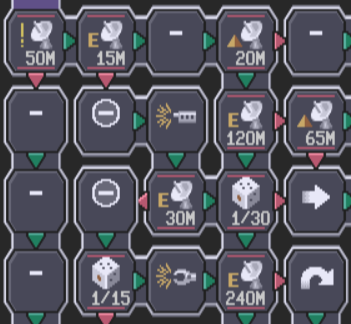
\includegraphics[width=0.5\textwidth]{img/CarnageHeartSoftware.png}
  \caption{Screenshot of the programming interface in Carnage Heart.\cite{carnageheartsoftware}}
  \label{fig:carnageheartsoftware}
\end{figure}

Carnage Heart teaches only basic programming constructs, but do not present them as such. Instead the player is presented with a set of rules, which are much like the rules of programming, and are told to create what is basically an AI for the robot.\todo{Do more such games exist? If so, maybe take in one more example and relate better to our game.}

This approach to teaching basic programming constructs is very relevant to our project, since our purpose is to make a similar game.